Analyzing conformance and performance expressed as averages over the whole model and log is very broad. Many real-life processes contain complex patterns and behavior as shown in the introduction. They can only be discovered when combining multiple perspectives on the data. The approach presented here focuses on localizing metrics for conformance, performance and process context to individual places in the Petri net model. The metrics are further localized to time intervals to make changes over time visible.

The approach consists of three steps:
\begin{enumerate}
    \item The log is projected onto the places of the process model to extract a \emph{locally mapped log}
    \item \emph{Interactions} are extracted from this \emph{locally mapped log}
    \item Metrics are calculated from \emph{interactions} for time intervals
\end{enumerate}

In the following, we introduce these steps in order.

\section{Locally mapping the log}
The first step requires some pre-processing. To properly handle the start and end places in the next steps, we insert unique start and end events into every trace. Their $activity$ is $\tstart$ or $\tend$ respectively. Their $time$ attribute is the time of first or last event respectively. Let $\E^\prime \supset \E$ be the universe of events including all artificial start and end marker events. To add the corresponding $\tstart$ and $\tend$ transitions in the model, a system net $SN=(PN,M_i,M_f)$ with initial and final marking is required. The $\tstart$ transition $t_{\tstart}$ is connected to all places in $M_i$ and the $\tend$ transition $t_{\tend}$ from all places in $M_f$. So for $PN = (P,T,F,l)$ the pre-processed Petri net is $PN^\prime=(P,T^\prime,F^\prime,l^\prime)$ with $F^\prime = F \cup \set{ (t_{\tstart},p) }{p\in M_i}\cup \set{(p,t_{\tend})}{p \in M_f}$, $T^\prime = T \cup \{t_{\tstart},t_{\tend}\}$, $\forall t\in T: l^\prime(t)=l(t)$ and $l^\prime(t_{\tstart}) = \tstart, l^\prime(t_{\tend})) = \tend$. Figure \ref{fig:preprocessednet} shows the pre-processed version of Figure \ref{fig:simplenet}.

\begin{figure}
    \centering
    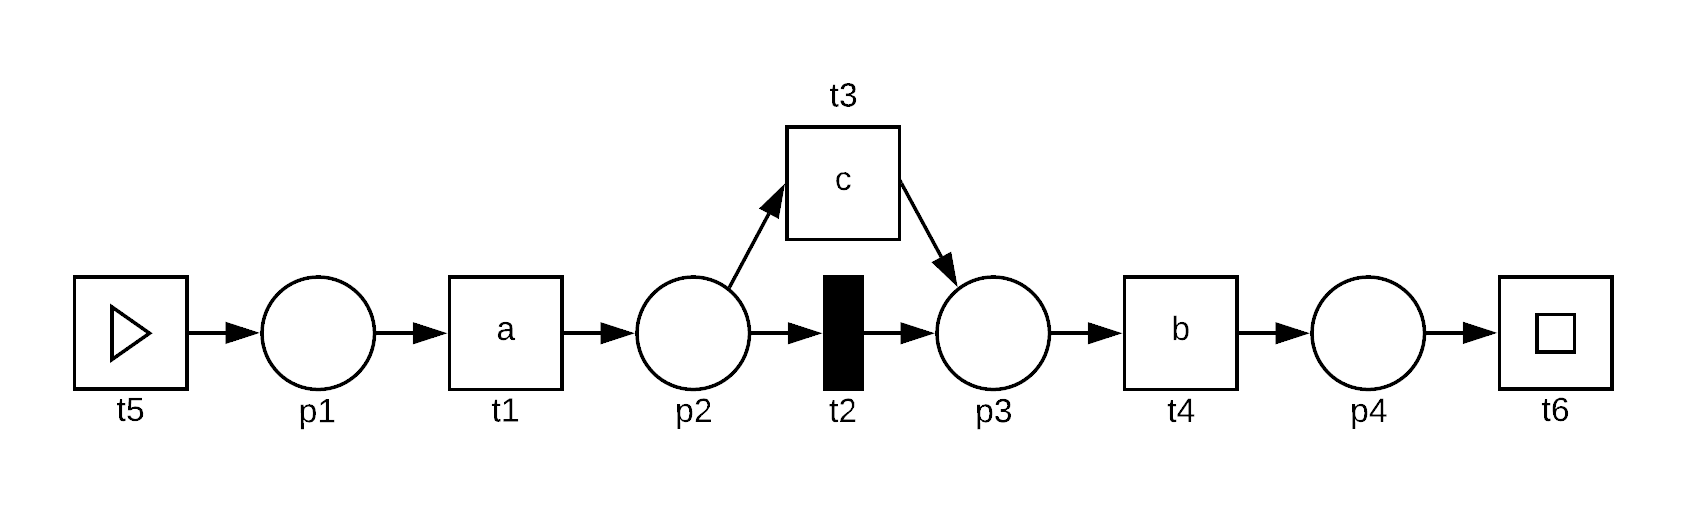
\includegraphics[width=0.6\textwidth]{figures/concept/preproc_simplenet.png}
    \caption{The simple model after pre-processing}
    \label{fig:preprocessednet}
\end{figure}

From this point on, we assume all Petri nets and logs to be pre-processed in this way.
We partition the adjacent transitions of a place into visible and invisible transitions, so for a place $p\in P$, $adj(p)=(\pre p \cup \post p) \cap T^{l}$ is the set of adjacent visible transitions and $adj_{\tau}(p) =(\pre p \cup \post p) \cap T^{\tau}$ is the set of adjacent silent transitions. To be able to add silent transition executions, let $l_{\tau}:T^{\tau} \to A_{\tau}$ be a labeling function which assigns a unique artificial activity to every otherwise unlabeled $\tau$-transition. To further define the silent execution events, let $\I$ be the universe of all artificial silent (hence not in $\E^\prime$) events whose $activity$ attribute is a silent activity. With these definitions, a locally mapped case can be defined. It is a mapping of events from a case to transitions adjacent to a particular place.
\begin{definition}[Locally mapped case]
Let $\Log \in \Univ L$ be a log and $PN = (P,T,F,l)$ be a Petri net. For a case $c\in \Log$ and place $p\in P$, a locally mapped case $lmc$ for $p$ inherits (and overloads) all attributes of $c$ except for the $trace$ attribute. Its trace is overloaded to a sequence of pairs of real events from $\hat{c}$ and inserted artificial silent events together with a fitting transition, i.e. $\hat{lmc}=trace(lmc)\in ((\E^\prime \times adj(p)) \cup (\I \times adj_{\tau}(p)))^*$. For every pair $(e,t)\in \E^\prime \times adj(p)$ or $(i,t^\prime)\in \I \times adj_{\tau}(p)$ in the sequence, the label of the transition has to match the activity of the event, i.e. $activity(e) = l(t)$ and $activity(i) = l_{\tau}(t^\prime)$. All events in the sequence have to be unique and ordered by $time$, so $\forall 1\le i<j \le |\hat{lmc}|, \hat{lmc}_i=(e,t), \hat{lmc}_j = (e^\prime,t^\prime): e\neq e^\prime \wedge time(e) \le time(e^\prime)$. Lastly, the projection onto real events is a subset of the original trace, i.e. $set(\hat{lmc}\restriction_1\restriction_{\E^\prime}) \subseteq set(\hat{c})$. If $|\hat{lmc}| = 0$, $lmc$ is called an empty locally mapped case which means the case did not interact with the place $p$.
\end{definition}
There are many ways to map a case onto the locally mapped cases, so we first define a generalized strategy. The strategy also determines the mandatory $time$ attribute of inserted silent events.
\begin{definition}[Case mapping strategy]
Let $\Log \in \Univ L$ be a log and $PN = (P,T,F,l)$ a Petri net. For any case $c\in \Log$, a case mapping strategy $\func{case\_map\_strat(c)} = (lmc_p)_{p \in P}$ creates a locally mapped case for each place $p\in P$. It needs to be consistent because a transition execution mapped in one of the locally mapped cases needs to be included in all the others also adjacent to the transition. So, $\forall p\in P \ \forall (e,t) \in set(\hat{lmc}_p) \ \forall p^\prime \in (\pre t \cup \post t): (e,t)\in set(\hat{lmc}_{p^\prime})$.
\end{definition}
Consistency can be achieved by first selecting a subset of events, mapping them to transitions, adding silent executions and then projecting them onto the adjacent transitions of the places.
Now, the entire event log can be mapped onto individual places with locally mapped logs.
\begin{definition}[Locally mapped log]
Let $\Log \in \Univ L$ be a log, $PN = (P,T,F,l)$ be a Petri net and $\func{map\_strat}$ be a case mapping strategy. Then a locally mapped log $\Log_p$ of place $p\in P$ is the set of all non-empty locally mapped cases, i.e. $\Log_p=\set{lmc}{lmc = \func{map\_strat(c)}_p \wedge |\hat{lmc}|\neq 0 \wedge c \in \Log }$.
\end{definition}

We propose a specific case mapping strategy $\func{sync\_strat}$ where a global execution is mapped locally. It uses alignments to be able to handle duplicate transitions and silent transition executions. 
The synchronous moves already provide a mapping of a subset of events from the trace to transitions in the model, so only the silent transition executions have to be added. This is done by replaying the synchronous and invisible moves on the model in a token-based manner. Synchronous moves are always executed, even if not enabled. Invisible moves are only executed if they are enabled, to be able to set their $time$ attribute which is the instant they are enabled. That means chains of silent events consistently shift the sojourn duration between two real events to the place at the end of the chain. The invisible move chains can be cut-off by non-invisible model moves, leaving the deviation of missing this event on the places adjacent to these non-invisible model moves.
This way, the locally mapped cases can be seen as a projection of the fitting parts of the event log onto locally mapped logs for each place.
A variant $\func{all\_strat}$ also tries to consider log moves which makes it unsuitable for models with duplicate transitions. It essentially treats log moves which can be mapped to a transition as synchronous moves, executing them unconditionally. More information from the log is used that way. Especially loops in a trace which cannot be mimicked by the model and hence end up being log moves can contribute to the analysis this way.

\begin{algorithm}[tb]
\begin{algorithmic}
\Require given $PN = (P,T,F,l)$
\State $\forall p\in P: lmc_p \gets$ new locally mapped case
\State $\forall p\in P: \hat{lmc}_p \gets \langle \rangle$
\State $M \gets$ new empty marking
\State $\var{lastMappedTime}: P \nrightarrow Time$
\Function{mapStrat}{alignment $\gamma$, boolean $\var{mapLogMoves}$}
    \For{$i = 1 : |\gamma|$}
        \If{$\gamma_i = (e,t) \wedge activity(a) = l(t)$} \Comment{sync move}
            \State \Call{handleTransition}{$e$, $t$}
        \ElsIf{$\gamma_i = (e, \gg)$} \Comment{log move}
            \If{$\var{mapLogMoves} \wedge \exists t\in T: l(t) = activity(e)$}
                \State \Call{handleTransition}{$e$, $t$}
            \EndIf
        \ElsIf{$\gamma_i = (\gg, t) \wedge l(t) = \tau$} \Comment{inv move}
            \If{$M[t\rangle$}
                \State $enabledAt \gets \max\{ \var{lastMappedTime}(p)| p\in \pre t \}$
                \State $e_{\tau} \gets$ new unique event
                \State $activity(e_{\tau}) \gets l_{\tau}(t)$
                \State $time(e_{\tau}) \gets enabledAt$
               \State \Call{handleTransition}{$e_{\tau}$, $t$}
            \EndIf
        \EndIf
    \EndFor
    \State \Return $(lmc_p)_{p\in P}$
\EndFunction
\Function{handleTransition}{event $e$, transition $t$}
    \State $M \gets (M \setminus \pre t) \uplus \post t$
    \ForAll{$p \in {\pre t \cup \post t}$}
        \State $\hat{lmc}_p \gets \hat{lmc}_p \cdot (e,t)$
        \If{$p \in \post t$}
            \State $\var{lastMappedTime}(p) \gets time(e)$    
        \EndIf
    \EndFor
\EndFunction
\end{algorithmic}
\caption{The proposed $\func{map\_strat}$}
\label{alg:mapstrat}
\end{algorithm}

A configurable algorithm for both variants is presented in Algorithm \ref{alg:mapstrat}. Provided an alignment $\gamma$ of a case, it steps through the sequence of moves and updates the locally mapped cases accordingly in the helper function \textsc{handleTransition}. It uses the partial function $\var{lastMappedTime}$ to track timestamps and a marking $M$ as an updated current marking. The transitions of synchronous moves and, if desired, mapped log moves are fired regardless if they are enabled. Invisible model moves are executed if they were actually enabled otherwise they are ignored. When they are executed, a unique new event is created and its mandatory attributes set. Then it is treated like any other transition execution.

As an example, consider the pre-processed log cases $\hat{c_1} = \langle e_{11}^\tstart, e_{12}^b, e_{13}^a, e_{14}^c, e_{15}^\tend \rangle$ and $\hat{c_2} = \langle e_{21}^\tstart, e_{22}^a, e_{23}^b, e_{24}^\tend \rangle \}$ in log $\Log = \{ c_1, c_2\}$ on the model given in Figure \ref{fig:preprocessednet}. The results of both strategies on this log are shown in Figure \ref{fig:mapstrats}. With $\func{sync\_strat}$, the unfitting event $e_{12}^b$ of the first case is not mapped which assigns that deviation to places $p3$ and $p4$. $\func{all\_strat}$ maps this event, which hides the problem from $p4$ and focuses it on $p3$ as swapped events.
\begin{figure}
    \centering
    \begin{tabular}{|l|c|}
    \hline
    Local log & $\func{sync\_strat}$  \\
    \hline
    $\Log_{p1}$ 
    & $\{ \langle (e_{11}^\tstart,t5),(e_{13}^a,t1) \rangle, \langle (e_{21}^\tstart,t5), (e_{22}^a,t1) \rangle \}$ 
     \\
    $\Log_{p2}$ 
    & $\{ \langle (e_{13}^a,t1), (e_{14}^c,t3) \rangle, \langle (e_{22}^a,t1),(e_{\tau}^{t2},t2) \rangle \}$ 
    \\
    $\Log_{p3}$ 
    & $\{ \langle (e_{14}^c,t3) \rangle, \langle (e_{\tau}^{t2},t2),(e_{23}^b, t4) \rangle \}$ 
    \\
    $\Log_{p4}$ 
    & $\{ \langle (e_{15}^\tend, t6) \rangle, \langle (e_{23}^b,t4),(e_{24}^\tend, t6) \rangle \}$ 
    \\
    \hline
    \hline
    Local log & $\func{all\_strat}$ \\
    \hline
    $\Log_{p1}$ & $\{ \langle (e_{11}^\tstart,t5),(e_{13}^a,t1) \rangle, \langle (e_{21}^\tstart,t5), (e_{22},a) \rangle \}$ \\
    $\Log_{p2}$ & $\{ \langle (e_{13}^a,t1), (e_{14}^c,t3) \rangle, \langle (e_{22}^a,t1),(e_{\tau}^{t2},t2) \rangle \}$ \\
    $\Log_{p3}$ & $\{ \langle (e_{12}^b,t4),(e_{14}^c,t3) \rangle, \langle (e_{\tau}^{t2},t2), (e_{23}^b,t4) \rangle \}$ \\
    $\Log_{p4}$ & $\{ \langle (e_{12}^b,t4),(e_{15}^\tend,t6) \rangle, \langle (e_{23}^b,t4),(e_{24}^\tend,t6) \rangle \}$ \\
    \hline
    \end{tabular}
    \caption{Comparison of local log mapping strategies}
    \label{fig:mapstrats}
\end{figure}

\section{Extracting Interactions}
The next step relies on the locally mapped logs to pair up input events with output events. During token-based replay, the execution of an input activity of a place will produce a token on it and the execution of an output activity of the place will eventually consume the token. This is a complete interaction. The time difference between token production and consumption on the place is called sojourn time. If the trace is not fitting perfectly, this results in places where a token will be missing or remaining. These cases are classified as incomplete interactions.
\begin{definition}[Complete interaction, incomplete interaction]
Let $PN = (P,T,F,l)$ be a Petri net and $\hat{lmc} = \langle \hat{lmc}_1, \hat{lmc}_2,\ldots, \hat{lmc}_n \rangle$ be the trace of a locally mapped case of $p\in P$. A complete interaction is a tuple $ci = ( (e,t), (e^\prime,t^\prime) )$ where $(e,t) = \hat{lmc}_i, (e^\prime, t^\prime) = \hat{lmc}_j$ such that $1\le i < j \le n$ and $t \in{\pre p}$ and $t^\prime \in{\post p}$. All interactions have a $start$, $end$ and $duration$ attribute. $start(ci) = time(e)$, $end(ci) = time(e^\prime)$ and $duration(ci) = end(ci) - start(ci)$. An incomplete interaction $ii$ is a tuple where the missing pair is replaced by $\missup$ or $\missdown$. So with $(e,t) \in set(\hat{lmc})$: $ii = (\missup, (e,t))$ for $t\in \post p$, $ii = ((e,t), \missdown)$ for $t\in \pre p$ and any of those for $t\in \pre p \cap \post p$. That means self loops can appear in two different incomplete interactions. The attributes are $start(ii)=end(ii)=time(e)$ and $duration(ii) = 0$. Additionally, interactions also further inherit (and overload) the case attributes of the locally mapped case.
\end{definition}
To extract these interactions in a sensible way, we define a generic interaction extraction strategy. This heuristic further maps the locally mapped cases to all contained interactions.
\begin{definition}[Interaction sets, interaction extraction strategy]
Let $PN = (P,T,F,l)$ be a Petri net and $lmc$ a locally mapped case of $p\in P$. $\CIS$ is called a complete interaction set and $\IIS$ an incomplete interaction set. An interaction extraction strategy $\func{extract\_strat_p(lmc)}=\var{(\CIS, \IIS)}$ for place $p$ has to partition all pairs $(e,t)\in set(\hat{lmc})$ into valid complete and incomplete interactions. Pairs with a self loop transition have to appear in two interactions because they first consume a token then produce one again. So, for all $1\le j \le  |\hat{lmc}|=n$ with $\hat{lmc}_j=(e,t)$ the following has to hold:
\begin{align}
    &t\in \pre p \implies (\exists!\ j < k \le n: (\hat{lmc}_j, \hat{lmc}_k)\in \CIS) \XOR ((\hat{lmc}_j,\missdown) \in \IIS) \label{eq:1}\\
    &t\in \post p \implies (\exists!\ 1\le i < j: (\hat{lmc}_i, \hat{lmc}_j)\in \CIS) \XOR ((\missup,\hat{lmc}_j) \in \IIS) \label{eq:2}
\end{align}
\end{definition}
 In other words, a self loop either is in two complete interactions, first as an output transition second as an input transition. Or just in one of those complete interactions and in one incomplete one, or both the input and the output transition part of incomplete interactions.
 We propose a basic algorithm for an $\func{extract\_strat}$ with Algorithm \ref{alg:extractstrat}. It performs a local token-based replay on the place where events which try to consume non-existent tokens and events which produce tokens that are never consumed are classified as incomplete interactions. It is also configurable by choosing the internal data structure which stores the producing events as either a stack or a queue. This determines the heuristic used to determine which overlapping events belong together. A small example illustrating the difference is given in Figure \ref{fig:stackqueue}. Complete Interactions are double headed arrows and incomplete ones are \texttimes. The queue matches the first producer with the first consumer while the stack matches the last producer with the first consumer.
\begin{algorithm}
\begin{algorithmic}
\Require given $PN=(P,T,F)$ and place $p\in P$
\Function{extractInteractions}{locally mapped case $lmc$}
    \State $\CIS \gets \{\}$
    \State $\IIS \gets \{\}$
    \State $\var{upTimes} \gets new(stack)$ \Comment{or $new(queue)$}
    \For{$i = 1 : |\hat{lmc}|$}
        \State $(e,t) \gets \hat{lmc}_i$
        \If{$t \in \post p$}
            \If{$empty(\var{upTimes})$}
                \State $\IIS \gets \IIS \cup (\missup,(e,t))$
            \Else
                \State $(e^\prime, t^\prime) \gets remove(\var{upTimes})$
                \State $\CIS \gets \CIS \cup ((e^\prime, t^\prime), (e,t))$
            \EndIf
        \EndIf
        \If{$t \in{\pre p}$}
            \State $add(upTimes, (e,t))$
        \EndIf
    \EndFor
    \If{not $empty(\var{upTimes})$}
        \ForAll{$(e,t) \in \var{upTimes}$}
            \State $\IIS \gets \IIS \cup ((e,t), \missdown)$
        \EndFor
    \EndIf
    \State \Return $(\CIS, \IIS)$
\EndFunction
\end{algorithmic}
\caption{The proposed $\func{extract\_strat}$}
\label{alg:extractstrat}
\end{algorithm}
\begin{figure}
    \centering
    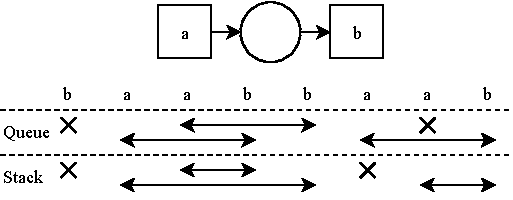
\includegraphics[scale=1]{figures/concept/overlap_strategy.pdf}
    \caption{A comparison of the queue and stack interaction extraction}
    \label{fig:stackqueue}
\end{figure}

Finally, the interaction sets for the local logs in Figure \ref{fig:mapstrats} of the running example are given in Figure \ref{fig:interactionstrats}. As mentioned before, $\func{sync\_strat}$ spreads out the incomplete interactions to all adjacent places while $\func{all\_strat}$ focuses it on the input places. Since swapped events can lead to two incomplete interactions, mapping log moves may lead to more incomplete interactions. In this example, using a stack or queue makes no difference.

\begin{figure}
    \centering
    \begin{tabular}{|l|c|c|}
    \hline
    \multirow{2}{*}{Local log} & \multicolumn{2}{|c|}{$\func{sync\_strat}$}  \\
     & $\CIS$ & $\IIS$ \\
    \hline
    $\Log_{p1}$ 
    & $\{ ((e_{11}^\tstart,t5),(e_{13}^a,t1)), ((e_{21}^\tstart,t5), (e_{22}^a,t1)) \}$ & $\{\}$ 
     \\
    $\Log_{p2}$ 
    & $\{ ((e_{13}^a,t1), (e_{14}^c,t3)), ((e_{22}^a,t1),(e_{\tau}^{t2},t2)) \}$ & $\{\}$ 
     \\
    $\Log_{p3}$ 
    & $\{ ((e_{\tau}^{t2},t2),(e_{23}^b, t4)) \}$ & $\{ ((e_{14}^c,t3),\missdown) \}$ 
     \\
    $\Log_{p4}$ 
    & $\{ ((e_{23}^b,t4),(e_{24}^\tend,t6)) \}$ & $\{ (\missup,(e_{15}^\tend,t6)) \}$
     \\
    \hline
    \hline
    \multirow{2}{*}{Local log} & \multicolumn{2}{|c|}{$\func{all\_strat}$} \\
    & $\CIS$ & $\IIS$ \\
    \hline
    $\Log_{p1}$ & $\{ ((e_{11}^\tstart,t5),(e_{13}^a,t1)), ((e_{21}^\tstart,t5), (e_{22}^a,t1)) \}$ & $\{\}$ \\
    $\Log_{p2}$ & $\{ ((e_{13}^a,t1), (e_{14}^c,t3)), ((e_{22}^a,t1),(e_{\tau}^{t2},t2)) \}$ & $\{\}$ \\
    $\Log_{p3}$ & $\{ ((e_{\tau}^{t2},t2),(e_{23}^b, t4)) \}$ & $\{ (\missup,(e_{23}^b,t4)), ((e_{14}^c, t3),\missdown) \}$ \\
    $\Log_{p4}$ & $\{ ((e_{12}^b,t4), (e_{15}^\tend,t6)), ((e_{23}^b,t4),(e_{24}^\tend,t6)) \}$ & $\{\}$ \\
    \hline
    \end{tabular}
    \caption{Continued running example with interaction sets}
    \label{fig:interactionstrats}
\end{figure}

\section{Time intervals} \label{timeintervals}
Until now, we extracted interactions of the log with places. This only uses the control-flow dimension and ordering of events. Since interactions also have the attributes $start$, $end$ and $duration$, it is possible to order them and spread them out over the time dimension. Complete interactions may also have a non-zero duration, so it is not trivial to filter them into time intervals. There are different types of overlap of an interaction with a time interval.
\begin{figure}
    \centering
    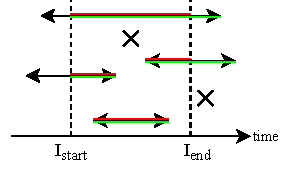
\includegraphics[scale=2]{figures/concept/timeinterval_overlap.pdf}
    \caption{Different types of overlap of interactions with a time interval}
    \label{fig:interactionoverlap}
\end{figure}
\begin{definition}[Time interval projections]
A time interval $[I_{start}, I_{end})$ has an inclusive start time $I_{start}$ and an exclusive end time $I_{end}$. The length of the interval is $L = I_{end} - I_{start}$.
The projections of an interaction set $\var{IS}$ ($\CIS$ or $\IIS$) to such a time interval are defined as functions with time interval parameters.
\begin{itemize}
    \item\emph{Touching}: $\mathit{T[I_{start}, I_{end})( IS ) = \set{int\in IS}{start(int) < I_{end} \wedge end(int)\ge I_{start}}}$
    \item\emph{StartingIn}: $\mathit{SI[I_{start}, I_{end})( IS ) = \set{int\in IS}{I_{start}\le start(int) < I_{end}}}$
    \item\emph{EndingIn}: $\mathit{EI[I_{start}, I_{end})( IS ) = \set{int\in IS}{I_{start}\le end(int) < I_{end}}}$
    \item\emph{ContainedIn}: $\mathit{CI[I_{start}, I_{end})( IS ) = \set{int\in IS}{I_{start}\le start(int) \le end(int) < I_{end}}}$
\end{itemize}
The actual overlap of a \emph{Touching} interaction $int \in \var{IS}$ with the time interval is between $\mathit{l\_limit = \max\{start(int), I_s\}}$ to $\mathit{r\_limit =  \min\{end(int), I_e\}}$, so $$\mathit{overlap[I_s,I_e)( int ) = \begin{cases} r\_limit - l\_limit & \text{if } start(int) < I_e \wedge end(int) \ge I_s  \\
0 & \text{otherwise}\end{cases}}$$
\end{definition}
Figure \ref{fig:interactionoverlap} shows some example interactions. The complete ones have arrowheads giving the $start$ and $end$ times and the incomplete ones are represented by \texttimes. All four complete ones are \emph{Touching}. The second one is also \emph{StartingIn}, the third one \emph{EndingIn} and the last one is both of those which makes it \emph{ContainedIn}. The top incomplete interaction is also everything while the bottom one is not touching at all. The overlap is colored red in the figure.

Finally, we define metrics for conformance, performance and process context.
For conformance, we propose two similar local fitness measures. One is based on the ratio of complete interactions and all interactions, while the other counts events instead of whole interactions. Since complete interactions are a pair of two events, the latter will always be higher, but it considers the actual time of occurrence more exactly.
\begin{definition}[Local fitness]
Let $\var{(CIS, IIS)}$ be a pair of sets of complete and incomplete interactions and $[I_s, I_e)$ be a time interval. The interactions starting in the interval are $\mathit{c\_start = SI[I_s, I_e)(\CIS)}$ and $\mathit{i\_start = SI[I_s, I_e)(IIS)}$ for complete and incomplete ones respectively.
$$\mathit{lfitness_{int}[I_s, I_e)( \CIS, \IIS ) = \begin{cases} \frac{|c\_start|}{|c\_start| + |i\_start|} & \text{if } |c\_start| + |i\_start| \neq 0\\
\text{undefined} & \text{otherwise}
\end{cases}}$$
The events from interactions inside the interval are $\var{ce\_start} = \set{e}{I_s \le time(e) < I_e \wedge e \in \set{e,e^\prime}{((e,t),(e^\prime,t^\prime))\in \CIS}}$ and $\var{ie\_start} = \set{e}{I_s \le time(e) < I_e \wedge ((e,t)) \in \IIS}$ for complete and incomplete interactions respectively.
$$\mathit{lfitness_{event}[I_s, I_e)( \CIS, \IIS ) = \begin{cases} \frac{|ce\_start|}{|ce\_start| + |ie\_start|} & \text{if } |ce\_start| + |ie\_start| \neq 0\\
\text{undefined} & \text{otherwise}
\end{cases}}$$
\end{definition}
If no interactions/events occur in the chosen time interval, the fitness is undefined. For the interval in Figure \ref{fig:interactionoverlap}, $\func{lfitness_{int}[I_{start}, I_{end})} = 0.67$ and $\func{lfitness_{event}[I_{start}, I_{end})} = 0.8$.

The current average sojourn time on a place is a measure for performance. The average is computed over complete interactions starting in the chosen interval. That means it is also undefined during intervals where no interactions occurred.
\begin{definition}[Local performance]
Let $\CIS$ be a set of complete interactions and $[I_s, I_e)$ be a time interval. Again, let $\mathit{c\_start = SI[I_s, I_e)(\CIS)}$.
$$\mathit{lperf[I_s,I_e)( \CIS ) = \begin{cases} \sum_{ci\in c\_start} duration(ci) / |c\_start| & \text{if } |c\_start|\neq 0\\
\text{undefined} & \text{otherwise} \end{cases}}$$
\end{definition}
$\func{lperf}$ describes how long (on average) cases that arrived at the place in the chosen interval eventually waited on there.

We propose three different metrics to try to measure the process context in terms of busyness at the current place during the chosen time interval. If many cases are currently waiting on this place, it will be busy.
\begin{definition}[Local busyness]
Let $\CIS$ be a set of complete interactions and $[I_s,I_e)$ be a time interval.
\begin{itemize}
    \item $\mathit{lbusyness_{c\_int}[I_s,I_e)( \CIS) = |SI[I_s,I_e)(CIS)|}$
    \item $\mathit{lbusyness_{activity}[I_s,I_e)( \CIS ) = \begin{cases} \sum_{ci \in CIS} overlap[I_s,I_e)(ci)/(I_e - I_s) & \text{if } I_s \neq I_e\\
    \text{undefined} & \text{otherwise} \end{cases}}$
    \item $\mathit{lbusyness_{remsojourn}[I_s,I_e)( \CIS ) = \sum_{ci\in T[I_s,I_e)(CIS)} (end(ci) - \max(start(ci),I_s))}$
\end{itemize}
\end{definition}

$\func{lbusyness_{c\_int}}$ is the number of complete interactions starting in the interval. Incomplete interactions may also inhibit performance since they are also in the log and actually occurred, so a variant $\func{lbusyness_{int}}$ counting all interactions may also be useful.
$\func{lbusyness_{activity}}$ is the sum of the ratios of overlap and the time interval size. The metric is relative to the interval size, so the interactions are weighed by their overlap which provides are more nuanced view on the busyness on a place during an interval. This is undefined for a time interval with the same start and end time.
$\func{lbusyness_{remsojourn}}$ is the total remaining sojourn time from the start of the interval of all touching interactions, shown in green in Figure \ref{fig:interactionoverlap}. In other words, if the place was a queue and could only handle one interaction after the other, it would take $\func{lbusyness_{remsojourn}}$ long to empty the queue. Instead of the total time, the average might also be interesting.

\section{Tying it all together} \label{alltogether}
The previous sections described the necessary process to arrive at metrics for conformance, performance and busyness. Given a system net $SN = (PN, M_i,M_f)$ and log $\Log$, the set of complete $\CIS$ and incomplete $\IIS$ interactions can be extracted for each individual place $p\in P$.
The metrics can then be calculated over time by dividing the whole process duration into a selected number of intervals or intervals of certain length like day, month or year. This yields a timeseries which can be used in statistical analysis to detect seasonality and trends.
By computing the relative standard deviation (standard deviation divided by mean) over the series or using other deviation metrics, one can also try to judge the stability of a certain metric over time. This way places can also be compared. Some might be in parts of the process that are quite streamlined and stable, while elsewhere the actual process execution may be more erratic in terms of conformance and performance. Figure \ref{fig:timeseriesschematic} shows a schematic of this on the running example model.
\begin{figure}
    \centering
    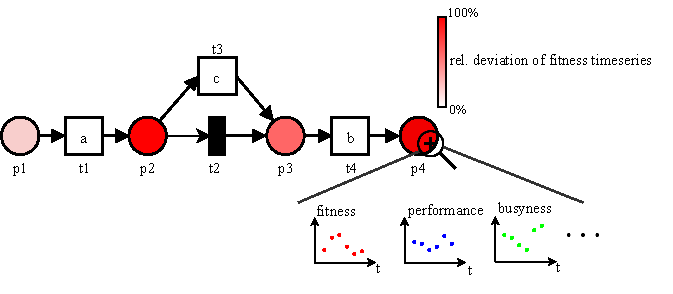
\includegraphics[width = \textwidth]{figures/concept/tyingtogether.pdf}
    \caption{Schematic result of applying the approach}
    \label{fig:timeseriesschematic}
\end{figure}
Another interesting application is finding correlations between these metrics. For example, does a high busyness value actually correlate with long sojourn times? In other words, how sensitive is this place to busyness? Or does a low conformance possibly lead to longer sojourn times? Since the $\CIS$ and $\IIS$ sets also contain the event and case data information, correlations can be extended to include those features. Which activity is often involved in incomplete interactions, and during which times? Do case attributes influence performance on this place? The localization of these questions to individual places and time frames makes it possible to find correlations which would be too weak to be detected over the whole log and process. For these purposes a dataset can be compiled containing all interactions with time and data information together with the metrics calculated for the duration of the interaction.

We also include another interesting aspect in our approach which is using the relative time since the case start. Every previously mentioned analysis can be performed for a relative time perspective by adjusting the intervals used for the metrics. It can be used to see after which time cases usually arrive at a place and if there are differences when they are later or earlier.